% Standalone figure: run make in this directory to build PDF and SVG.
\documentclass[11pt,tikz,border=0pt]{standalone}
\usepackage{fontspec}
\IfFontExistsTF{Helvetica Neue Light}{
  \setsansfont{Helvetica Neue Light}[BoldFont={Helvetica Neue Medium}]
  \newfontfamily\vnmedium{Helvetica Neue Medium}
}{
  \setsansfont{TeX Gyre Heros}
  \newcommand{\vnmedium}{\bfseries}
}
\renewcommand{\familydefault}{\sfdefault}
\usepackage{amsmath,amssymb,mathtools}
\usepackage{unicode-math}
\setmathfont{latinmodern-math.otf}
\usetikzlibrary{arrows.meta,calc,positioning}
\definecolor{vnslideink}{HTML}{333333}
\definecolor{vnslidebody}{HTML}{5E5E5E}
\definecolor{vnaccent}{HTML}{FF644E}
\definecolor{vnslidelink}{HTML}{579ACA}
\pagecolor{white}


\definecolor{bpLeftFill}{HTML}{C8E9F2}
\definecolor{bpLeftStroke}{HTML}{58A9C1}
\definecolor{bpLeftGroup}{HTML}{F1FAFC}
\definecolor{bpRightFill}{HTML}{FFDC91}
\definecolor{bpRightStroke}{HTML}{D89A29}
\definecolor{bpRightGroup}{HTML}{FFF9ED}
\definecolor{bpMatch}{HTML}{EF4136}
\begin{document}
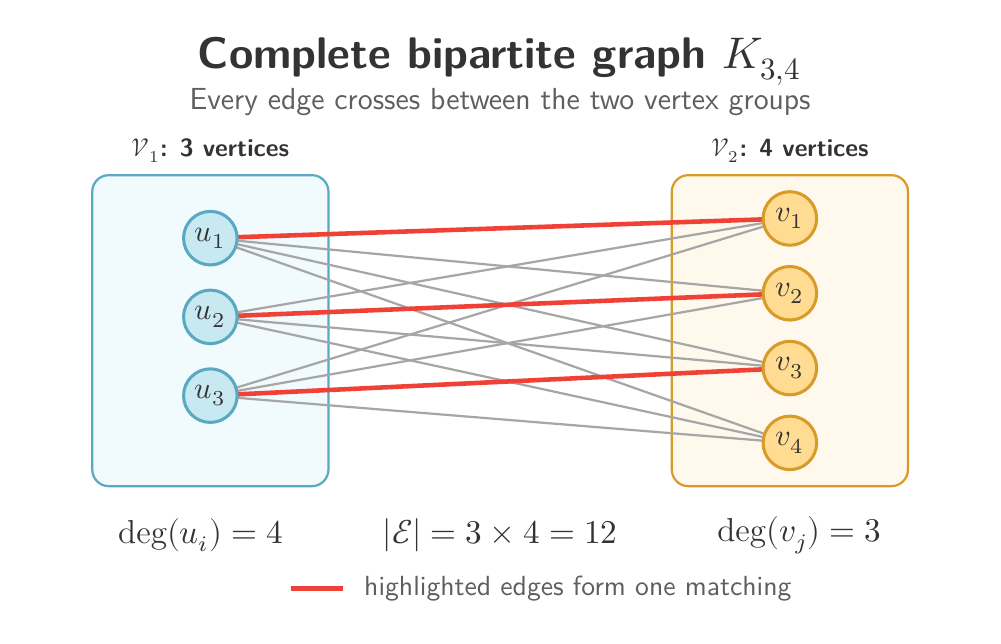
\begin{tikzpicture}[x=1cm,y=1cm,
  font=\sffamily\fontsize{11}{13}\selectfont,text=vnslideink,
  bpvertex/.style={circle,minimum size=6.8mm,inner sep=0pt,line width=1.1pt},
  bpgroup/.style={rounded corners=6pt,line width=0.8pt},
  bpmetric/.style={font=\fontsize{12}{14}\selectfont}]
  % The slide uses the panel export; the notebook uses the full heading.
  \ifdefined\BipartiteGraphOmitHeading
    \fill[white] (0,-0.35) rectangle (12,5.75);
    \path[use as bounding box] (0,-0.35) rectangle (12,5.75);
  \else
    \fill[white] (0,-0.35) rectangle (12,7.1);
    \node[font=\sffamily\bfseries\fontsize{16}{19}\selectfont] at (6,6.7)
      {Complete bipartite graph $K_{3,4}$};
    \node[text=vnslidebody] at (6,6.18)
      {Every edge crosses between the two vertex groups};
    \path[use as bounding box] (0,-0.35) rectangle (12,7.1);
  \fi

  \draw[bpgroup,draw=bpLeftStroke,fill=bpLeftGroup] (0.82,1.3) rectangle (3.82,5.25);
  \draw[bpgroup,draw=bpRightStroke,fill=bpRightGroup] (8.18,1.3) rectangle (11.18,5.25);
  \node[anchor=south,inner sep=0pt,font=\sffamily\bfseries\fontsize{9}{11}\selectfont] at (2.32,5.4) {$\mathcal V_1$: 3 vertices};
  \node[anchor=south,inner sep=0pt,font=\sffamily\bfseries\fontsize{9}{11}\selectfont] at (9.68,5.4) {$\mathcal V_2$: 4 vertices};

  \foreach \i/\y in {1/4.45,2/3.45,3/2.45}
    {\coordinate (u\i) at (2.32,\y);}
  \foreach \j/\y in {1/4.7,2/3.75,3/2.8,4/1.85}
    {\coordinate (v\j) at (9.68,\y);}
  % All twelve edges are present; u1-v1, u2-v2, and u3-v3 form the matching.
  \foreach \i in {1,2,3}
    {\foreach \j in {1,2,3,4}
      {\draw[draw=vnslidebody!55,line width=0.8pt] (u\i)--(v\j);}}
  \foreach \i in {1,2,3}
    {\draw[draw=bpMatch,line width=1.65pt] (u\i)--(v\i);}
  \foreach \i in {1,2,3}
    {\node[bpvertex,draw=bpLeftStroke,fill=bpLeftFill] at (u\i) {$u_{\i}$};}
  \foreach \j in {1,2,3,4}
    {\node[bpvertex,draw=bpRightStroke,fill=bpRightFill] at (v\j) {$v_{\j}$};}

  \node[bpmetric] at (2.2,0.68) {$\deg(u_i)=4$};
  \node[bpmetric] at (6,0.68) {$|\mathcal E|=3\times4=12$};
  \node[bpmetric] at (9.8,0.68) {$\deg(v_j)=3$};
  \draw[draw=bpMatch,line width=1.65pt] (3.35,0)--(4,0);
  \node[anchor=west,text=vnslidebody,font=\sffamily\fontsize{10}{12}\selectfont]
    at (4.15,0) {highlighted edges form one matching};
\end{tikzpicture}
\end{document}
